\documentclass[10pt]{article}
\usepackage{icmlko}

\icmlmeta{IP 파운데이션 월드모델}{85}{판에 올라온 것을 집을 자가 없다}{신경망은 또 졌고 결측 대입은 문턱에 못 미쳤다 --- 그러나 얼마가 걸려 있는지는 정확히 쟀다}

\begin{document}

\twocolumn[
\icmlheader

\begin{abstract}
노트 84가 병목을 구조로 지목했다 --- 직전작 성적(단일 상관 최대 $+$0.709)이
\texttt{min\_cov=0.6} 문턱에 걸려 통째로 버려진다. 얼마가 걸려 있는지부터
정확히 쟀다. 같은 레코드 집합에서 재면 \textbf{$+$0.4501$\to+$0.4735}
($\Delta+$0.0234)이고, 모바일은 $+$0.645에서 \textbf{$+$0.803}으로 간다.
그다음 셋을 시도했다. \textbf{첫째, 마스크를 입력으로 받는 인코더}(노트 60--62의
재대결) --- 값 여섯 $+$ 마스크 여섯, 공유 MLP, 복원 손실. \textbf{또 진다}
($+$0.3575 대 현행 $+$0.4038). 잠재 차원과 복원 비중을 바꿔도 $+$0.32$\sim+$0.36이다.
어디서 지는지가 분명하다 --- \textbf{작은 도메인이 무너진다}(아이돌 $+$0.473$\to+$0.161,
애니 $+$0.274$\to+$0.156). 진단: 공유 인코더는 \textbf{쌍별 정렬 자유도를
포기}한다. 노트 40이 전역 정렬을 버리고 쌍별로 간 이유가 그것이었다.
\textbf{둘째, \texttt{min\_cov} 를 내리는 것} --- 표본이 11,546에서 5,986으로
무너져 비교가 성립하지 않는다. \textbf{셋째, 결측 표시자 방법}(값은 중립 대입,
표시자는 별도 축) --- 구조를 안 바꾸고 표본 손실 0으로 \textbf{$+$0.4178}
($\Delta+$0.0140)이다. 그런데 짝지은 구간이 \textbf{0/4 씨앗}에서 0을 포함한다.
\textbf{셋 다 문턱을 못 넘었다.} 직전작 성적은 판에 올라와 있고 아직 아무 자도
그것을 집어 올리지 못한다.
\end{abstract}
]

\begin{figure*}[t]
\centering
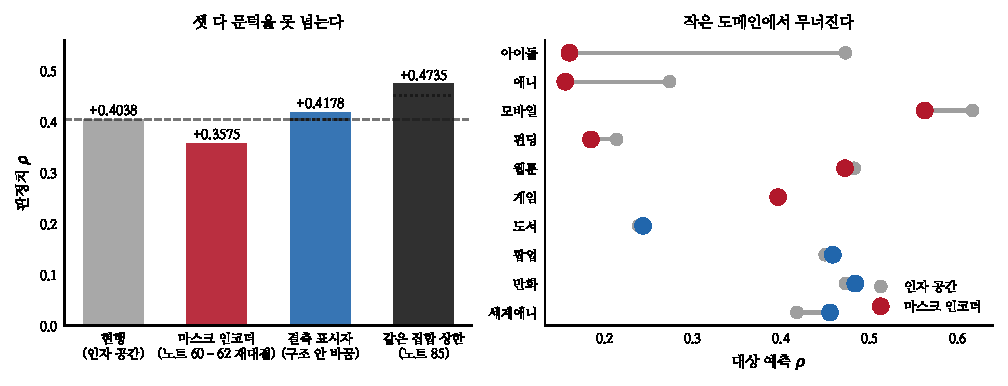
\includegraphics[width=\textwidth]{figs/enc.pdf}
\caption{왼쪽 --- 세 접근의 판정치. 오른쪽 --- 마스크 인코더의 대상별 승패.}
\end{figure*}

\section{얼마가 걸려 있나}

노트 84는 ``관측된 곳에서만'' 재서 표본이 달랐다. 같은 레코드 집합에서 다시
잰다 --- 직전작이 관측된 레코드만 남기고 축이 있을 때와 없을 때를 비교한다.

\begin{table}[t]
\centering\tsize
\caption{같은 레코드 집합. 직전작 축 없이 대 넣고.}
\begin{tabular}{lrrr}
\toprule
대상 & 없이 & 넣고 & $\Delta$ \\
\midrule
\textbf{모바일} & $+$0.6449 & \textbf{$+$0.8029} & $+$0.1580 \\
펀딩 & $+$0.4474 & $+$0.5833 & $+$0.1359 \\
게임 & $+$0.4654 & $+$0.5195 & $+$0.0540 \\
웹툰 & $+$0.4767 & $+$0.5190 & $+$0.0424 \\
팝업 & $+$0.4527 & $+$0.4648 & $+$0.0121 \\
만화 & $+$0.5124 & $+$0.4894 & $-$0.0230 \\
\textbf{애니} & $+$0.3544 & $+$0.2515 & $-$0.1028 \\
\midrule
\textbf{평균} & \textbf{$+$0.4501} & \textbf{$+$0.4735} & $+$0.0234 \\
\bottomrule
\end{tabular}
\end{table}

열 중 다섯이 오르고 다섯이 내려 평균 $+$0.0234다. 모바일이 $+$0.8029로 노트
83의 라벨 천장 추정(0.72$\sim$0.75)을 넘는다.

\section{마스크 인코더 --- 또 졌다}

\begin{quote}\fontsize{9.5}{11.5}\selectfont
\textbf{설계.} 입력은 값 여섯 $+$ 마스크 여섯 = 12차원(결측은 0, 마스크가 알린다).
공유 MLP 12$\to$32$\to$16$\to$2로 잠재를 뽑고, 디코더 2$\to$12로 관측된 자리만
복원한다. 도메인별 선형 머리가 표준화 라벨을 맞히고, 대상 도메인은 \emph{라벨
지도만} 뺀다. \textbf{공유 인코더라 프로크루스테스가 없다.}
\end{quote}

\begin{table}[t]
\centering\tsize
\caption{설정을 바꿔도.}
\begin{tabular}{lrr}
\toprule
잠재 차원 & 복원 비중 & 판정치 \\
\midrule
2 & 0.50 & $+$0.3575 \\
2 & 0.05 & $+$0.3240 \\
3 & 0.50 & $+$0.3392 \\
3 & 0.05 & $+$0.3428 \\
\midrule
\multicolumn{2}{l}{현행 인자 공간} & \textbf{$+$0.4038} \\
\bottomrule
\end{tabular}
\end{table}

\claimx{공유 인코더는 쌍별 정렬 자유도를 포기하기 때문에 진다. 대상별로 보면
큰 도메인(만화 · 세계애니 · 팝업)에서는 이기고 \textbf{작은 도메인에서 무너진다}
--- 아이돌 $+$0.473$\to+$0.161, 애니 $+$0.274$\to+$0.156.}{손실은 도메인별
평균이라 큰 도메인이 지배하지 않는다. 그런데도 작은 도메인이 무너지므로 원인은
표본 가중이 아니라 표현의 자유도로 보이는데, 갈라 확인하지 않았다.}

노트 40이 전역 정렬(모두를 팝업에 맞춤)을 버리고 쌍별 정렬로 간 이유가 정확히
이것이었다 --- 도메인마다 관측 축이 다르므로 하나의 공간에 다 밀어 넣으면
어느 하나가 희생된다. 인코더는 그 전역 정렬을 학습으로 다시 하는 셈이다.

\section{결측 표시자 --- 문턱 바로 아래}

\begin{table}[t]
\centering\tsize
\caption{구조를 안 바꾸는 세 변형. 레코드 11,546건 그대로.}
\begin{tabular}{lrr}
\toprule
& $\rho$ & $\Delta$ \\
\midrule
현행 & $+$0.4038 & --- \\
값만(중립 대입) & $+$0.4160 & $+$0.0122 \\
값$+$표시자 & $+$0.4141 & $+$0.0103 \\
\textbf{값$+$표시자(공통 축)} & \textbf{$+$0.4178} & \textbf{$+$0.0140} \\
\bottomrule
\end{tabular}
\end{table}

\texttt{factor\_space} 가 완전 케이스만 쓰므로 덮개율 36\%인 축은 못 쓴다.
그런데 \textbf{값과 표시자를 나눠 두 열로 넣으면} 둘 다 덮개율 100\%가 된다 ---
관측되면 백분위, 아니면 0.5(중립), 표시자가 관측 여부를 알린다. 노트 35 · 37이
금지한 것은 \emph{결측을 관측값인 척하는 것}인데, 표시자가 함께 있으면 모형이
구별할 수 있다.

\begin{table}[t]
\centering\tsize
\caption{채택 검정. 씨앗 넷, 붓스트랩 120회.}
\begin{tabular}{lrl}
\toprule
씨앗 & $\Delta$ & 95\% 구간 \\
\midrule
20260729 & $+$0.0088 & $[-0.0065, +0.0214]$ \\
19770101 & $+$0.0101 & $[-0.0097, +0.0229]$ \\
20250315 & $+$0.0100 & $[-0.0063, +0.0209]$ \\
20260101 & $+$0.0098 & $[-0.0090, +0.0235]$ \\
\midrule
\multicolumn{2}{l}{채택} & \textbf{0/4} \\
\bottomrule
\end{tabular}
\end{table}

\claimx{결측 표시자 방법이 표본 손실 없이 $+$0.0140을 내지만 짝지은 구간이 네
씨앗 전부에서 0을 포함한다. \textbf{채택하지 않는다.}}{$+$0.0140은 구간 반폭
(0.033)의 절반이 안 된다. 도메인이 더 늘어 반폭이 0.02 아래가 되면 통과할 수
있다 --- 노트 83이 도메인은 정밀도를 산다고 한 것이 여기서 값을 한다.}

\section{셋 다 못 집었다}

\begin{table}[t]
\centering\tsize
\caption{시도 요약.}
\begin{tabular}{lrl}
\toprule
& $\rho$ & \\
\midrule
현행 인자 공간 & $+$0.4038 & --- \\
마스크 인코더 & $+$0.3575 & 악화 \\
\texttt{min\_cov} 내리기 & --- & 표본 붕괴 \\
결측 표시자 & $+$0.4178 & 0/4 채택 \\
\midrule
\textbf{같은 집합 상한} & \textbf{$+$0.4735} & 판에 올라온 몫 \\
\bottomrule
\end{tabular}
\end{table}

직전작 성적은 판에 올라와 있다. 같은 레코드에서 재면 $+$0.0234가 있고, 모바일
하나에서는 $+$0.158이다. \textbf{그런데 지금 가진 어느 자도 그것을 집어 올리지
못한다} --- 인자 공간은 문턱에서 버리고, 표시자로 우회하면 문턱에 0.014 모자라고,
인코더는 그 대가로 쌍별 정렬을 잃는다.

\section{한계}

\begin{itemize}[leftmargin=1.1em,itemsep=0.15em]
\item 인코더를 네 설정만 봤다. 층 수 · 폭 · 학습률 · 정규화를 안 훑었다.
\item 인코더가 작은 도메인에서 무너지는 이유를 ``정렬 자유도''로 설명했는데
      확인 실험을 안 했다. 도메인별 어댑터를 붙여 보면 갈릴 것이다.
\item 중립값을 0.5로 뒀다. 도메인 중앙값이나 다른 값이면 다를 수 있다.
\item 직전작 성적이 대상 라벨(다른 레코드의)을 쓴다. 새 카테고리에는 못 쓴다.
\item 팝업에는 창작자/IP 키가 없어 직전작 성적을 못 만들었다. 제품에서 가장
      값진 자리인데 계속 못 재고 있다.
\end{itemize}

\section{다음}

\begin{enumerate}[leftmargin=1.3em,itemsep=0.15em]
\item \textbf{인코더에 도메인별 어댑터를 붙인다} --- 공유 인코더 뒤에 도메인마다
      작은 선형 변환을 두면 쌍별 정렬의 자유도를 되찾는다. 진단이 맞는지
      가르는 실험이다.
\item 팝업 레코드에 IP/브랜드 키를 붙인다. 직전작 성적을 팝업에서 만들 수 있으면
      제품 수치가 직접 오른다.
\item 결측 표시자를 보류로 두고, 도메인이 늘어 반폭이 0.02 아래가 되면 다시
      판정한다.
\item 중립값을 도메인 중앙값으로 바꿔 본다.
\end{enumerate}

\vspace{0.6em}
\hrule height 0.3pt
\vspace{0.5em}
{\footnotesize
\textbf{참고문헌}\\[0.3em]
Little, R. J. A., Rubin, D. B. (2019). \emph{Statistical Analysis with Missing
Data}, 3rd ed. Wiley.\\[0.15em]
Josse, J. et al. (2019). On the consistency of supervised learning with missing
values. \emph{arXiv:1902.06931}.\\[0.15em]
Schoenemann, P. H. (1966). A generalized solution of the orthogonal Procrustes
problem. \emph{Psychometrika}, 31(1), 1--10.\\[0.15em]
Grinsztajn, L. et al. (2022). Why do tree-based models still outperform deep
learning on typical tabular data? \emph{NeurIPS}.\\[0.15em]
Rebuffi, S.-A. et al. (2017). Learning multiple visual domains with residual
adapters. \emph{NIPS}, 506--516.
}

\end{document}
